% Created by tikzDevice version 0.12.3.1 on 2022-03-24 13:38:39
% !TEX encoding = UTF-8 Unicode
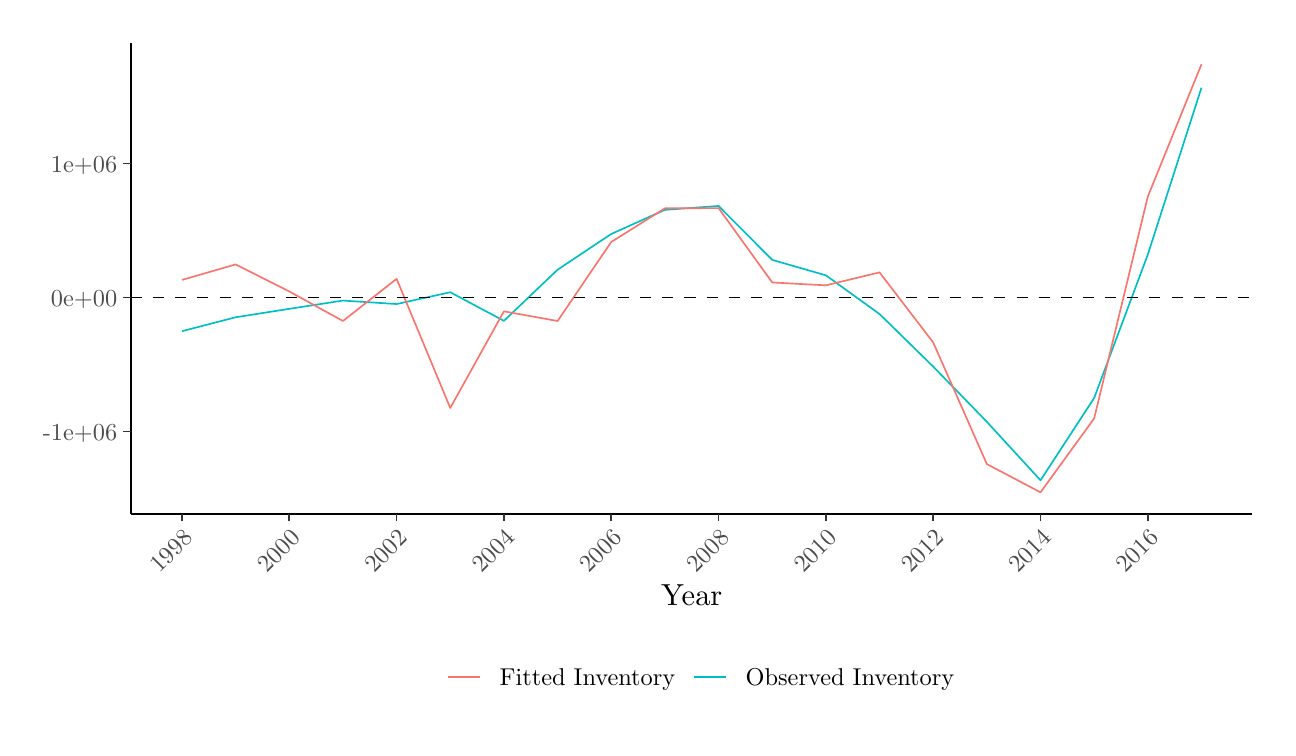
\begin{tikzpicture}[x=1pt,y=1pt]
\definecolor{fillColor}{RGB}{255,255,255}
\path[use as bounding box,fill=fillColor,fill opacity=0.00] (0,0) rectangle (448.07,252.94);
\begin{scope}
\path[clip] (  0.00,  0.00) rectangle (448.07,252.94);
\definecolor{drawColor}{RGB}{255,255,255}
\definecolor{fillColor}{RGB}{255,255,255}

\path[draw=drawColor,line width= 0.6pt,line join=round,line cap=round,fill=fillColor] (  0.00,  0.00) rectangle (448.07,252.94);
\end{scope}
\begin{scope}
\path[clip] ( 37.33, 77.31) rectangle (442.57,247.44);
\definecolor{fillColor}{RGB}{255,255,255}

\path[fill=fillColor] ( 37.33, 77.31) rectangle (442.57,247.44);
\definecolor{drawColor}{RGB}{0,191,196}

\path[draw=drawColor,line width= 0.6pt,line join=round] ( 55.75,143.26) --
	( 75.14,148.29) --
	( 94.53,151.34) --
	(113.92,154.33) --
	(133.31,153.07) --
	(152.70,157.34) --
	(172.09,147.00) --
	(191.48,165.48) --
	(210.87,178.39) --
	(230.26,187.11) --
	(249.65,188.51) --
	(269.04,169.03) --
	(288.43,163.45) --
	(307.82,149.46) --
	(327.21,130.47) --
	(346.60,110.52) --
	(365.99, 89.38) --
	(385.37,119.13) --
	(404.76,170.95) --
	(424.15,231.25);
\definecolor{drawColor}{RGB}{248,118,109}

\path[draw=drawColor,line width= 0.6pt,line join=round] ( 55.75,161.78) --
	( 75.14,167.39) --
	( 94.53,157.62) --
	(113.92,146.95) --
	(133.31,162.18) --
	(152.70,115.52) --
	(172.09,150.44) --
	(191.48,146.94) --
	(210.87,175.50) --
	(230.26,187.66) --
	(249.65,187.74) --
	(269.04,160.87) --
	(288.43,159.83) --
	(307.82,164.51) --
	(327.21,139.19) --
	(346.60, 95.24) --
	(365.99, 85.04) --
	(385.37,111.73) --
	(404.76,191.89) --
	(424.15,239.71);
\definecolor{drawColor}{RGB}{0,0,0}

\path[draw=drawColor,line width= 0.6pt,dash pattern=on 4pt off 4pt ,line join=round] ( 37.33,155.39) -- (442.57,155.39);
\end{scope}
\begin{scope}
\path[clip] (  0.00,  0.00) rectangle (448.07,252.94);
\definecolor{drawColor}{RGB}{0,0,0}

\path[draw=drawColor,line width= 0.6pt,line join=round] ( 37.33, 77.31) --
	( 37.33,247.44);
\end{scope}
\begin{scope}
\path[clip] (  0.00,  0.00) rectangle (448.07,252.94);
\definecolor{drawColor}{gray}{0.30}

\node[text=drawColor,anchor=base east,inner sep=0pt, outer sep=0pt, scale=  0.88] at ( 32.38,103.94) {-1e+06};

\node[text=drawColor,anchor=base east,inner sep=0pt, outer sep=0pt, scale=  0.88] at ( 32.38,152.36) {0e+00};

\node[text=drawColor,anchor=base east,inner sep=0pt, outer sep=0pt, scale=  0.88] at ( 32.38,200.78) {1e+06};
\end{scope}
\begin{scope}
\path[clip] (  0.00,  0.00) rectangle (448.07,252.94);
\definecolor{drawColor}{gray}{0.20}

\path[draw=drawColor,line width= 0.6pt,line join=round] ( 34.58,106.97) --
	( 37.33,106.97);

\path[draw=drawColor,line width= 0.6pt,line join=round] ( 34.58,155.39) --
	( 37.33,155.39);

\path[draw=drawColor,line width= 0.6pt,line join=round] ( 34.58,203.81) --
	( 37.33,203.81);
\end{scope}
\begin{scope}
\path[clip] (  0.00,  0.00) rectangle (448.07,252.94);
\definecolor{drawColor}{RGB}{0,0,0}

\path[draw=drawColor,line width= 0.6pt,line join=round] ( 37.33, 77.31) --
	(442.57, 77.31);
\end{scope}
\begin{scope}
\path[clip] (  0.00,  0.00) rectangle (448.07,252.94);
\definecolor{drawColor}{gray}{0.20}

\path[draw=drawColor,line width= 0.6pt,line join=round] ( 55.75, 74.56) --
	( 55.75, 77.31);

\path[draw=drawColor,line width= 0.6pt,line join=round] ( 94.53, 74.56) --
	( 94.53, 77.31);

\path[draw=drawColor,line width= 0.6pt,line join=round] (133.31, 74.56) --
	(133.31, 77.31);

\path[draw=drawColor,line width= 0.6pt,line join=round] (172.09, 74.56) --
	(172.09, 77.31);

\path[draw=drawColor,line width= 0.6pt,line join=round] (210.87, 74.56) --
	(210.87, 77.31);

\path[draw=drawColor,line width= 0.6pt,line join=round] (249.65, 74.56) --
	(249.65, 77.31);

\path[draw=drawColor,line width= 0.6pt,line join=round] (288.43, 74.56) --
	(288.43, 77.31);

\path[draw=drawColor,line width= 0.6pt,line join=round] (327.21, 74.56) --
	(327.21, 77.31);

\path[draw=drawColor,line width= 0.6pt,line join=round] (365.99, 74.56) --
	(365.99, 77.31);

\path[draw=drawColor,line width= 0.6pt,line join=round] (404.76, 74.56) --
	(404.76, 77.31);
\end{scope}
\begin{scope}
\path[clip] (  0.00,  0.00) rectangle (448.07,252.94);
\definecolor{drawColor}{gray}{0.30}

\node[text=drawColor,rotate= 45.00,anchor=base east,inner sep=0pt, outer sep=0pt, scale=  0.88] at ( 60.04, 68.07) {1998};

\node[text=drawColor,rotate= 45.00,anchor=base east,inner sep=0pt, outer sep=0pt, scale=  0.88] at ( 98.82, 68.07) {2000};

\node[text=drawColor,rotate= 45.00,anchor=base east,inner sep=0pt, outer sep=0pt, scale=  0.88] at (137.60, 68.07) {2002};

\node[text=drawColor,rotate= 45.00,anchor=base east,inner sep=0pt, outer sep=0pt, scale=  0.88] at (176.38, 68.07) {2004};

\node[text=drawColor,rotate= 45.00,anchor=base east,inner sep=0pt, outer sep=0pt, scale=  0.88] at (215.15, 68.07) {2006};

\node[text=drawColor,rotate= 45.00,anchor=base east,inner sep=0pt, outer sep=0pt, scale=  0.88] at (253.93, 68.07) {2008};

\node[text=drawColor,rotate= 45.00,anchor=base east,inner sep=0pt, outer sep=0pt, scale=  0.88] at (292.71, 68.07) {2010};

\node[text=drawColor,rotate= 45.00,anchor=base east,inner sep=0pt, outer sep=0pt, scale=  0.88] at (331.49, 68.07) {2012};

\node[text=drawColor,rotate= 45.00,anchor=base east,inner sep=0pt, outer sep=0pt, scale=  0.88] at (370.27, 68.07) {2014};

\node[text=drawColor,rotate= 45.00,anchor=base east,inner sep=0pt, outer sep=0pt, scale=  0.88] at (409.05, 68.07) {2016};
\end{scope}
\begin{scope}
\path[clip] (  0.00,  0.00) rectangle (448.07,252.94);
\definecolor{drawColor}{RGB}{0,0,0}

\node[text=drawColor,anchor=base,inner sep=0pt, outer sep=0pt, scale=  1.10] at (239.95, 44.09) {Year};
\end{scope}
\begin{scope}
\path[clip] (  0.00,  0.00) rectangle (448.07,252.94);
\definecolor{fillColor}{RGB}{255,255,255}

\path[fill=fillColor] (139.59,  5.50) rectangle (340.31, 30.95);
\end{scope}
\begin{scope}
\path[clip] (  0.00,  0.00) rectangle (448.07,252.94);
\definecolor{drawColor}{RGB}{248,118,109}

\path[draw=drawColor,line width= 0.6pt,line join=round] (152.04, 18.23) -- (163.60, 18.23);
\end{scope}
\begin{scope}
\path[clip] (  0.00,  0.00) rectangle (448.07,252.94);
\definecolor{drawColor}{RGB}{248,118,109}

\path[draw=drawColor,line width= 0.6pt,line join=round] (152.04, 18.23) -- (163.60, 18.23);
\end{scope}
\begin{scope}
\path[clip] (  0.00,  0.00) rectangle (448.07,252.94);
\definecolor{drawColor}{RGB}{0,191,196}

\path[draw=drawColor,line width= 0.6pt,line join=round] (240.94, 18.23) -- (252.50, 18.23);
\end{scope}
\begin{scope}
\path[clip] (  0.00,  0.00) rectangle (448.07,252.94);
\definecolor{drawColor}{RGB}{0,191,196}

\path[draw=drawColor,line width= 0.6pt,line join=round] (240.94, 18.23) -- (252.50, 18.23);
\end{scope}
\begin{scope}
\path[clip] (  0.00,  0.00) rectangle (448.07,252.94);
\definecolor{drawColor}{RGB}{0,0,0}

\node[text=drawColor,anchor=base west,inner sep=0pt, outer sep=0pt, scale=  0.88] at (170.55, 15.20) {Fitted Inventory};
\end{scope}
\begin{scope}
\path[clip] (  0.00,  0.00) rectangle (448.07,252.94);
\definecolor{drawColor}{RGB}{0,0,0}

\node[text=drawColor,anchor=base west,inner sep=0pt, outer sep=0pt, scale=  0.88] at (259.44, 15.20) {Observed Inventory};
\end{scope}
\end{tikzpicture}
